% #######################################
% ########### FILL THESE IN #############
% #######################################
\def\mytitle{Tic-Tac-Toe Coursework Report}
\def\myauthor{Maria Luque Anguita}
\def\contact{40280156@napier.ac.uk}
\def\mymodule{Algorithms and Data Structures (SET08122)}
% #######################################
% #### YOU DON'T NEED TO TOUCH BELOW ####
% #######################################
\documentclass[10pt, a4paper]{article}
\usepackage[a4paper,outer=1.5cm,inner=1.5cm,top=1.75cm,bottom=1.5cm]{geometry}
\twocolumn
\usepackage{graphicx}
\graphicspath{{./images/}}
%colour our links, remove weird boxes
\usepackage[colorlinks,linkcolor={black},citecolor={blue!80!black},urlcolor={blue!80!black}]{hyperref}
%Stop indentation on new paragraphs
\usepackage[parfill]{parskip}
%% Arial-like font
\IfFileExists{uarial.sty}
{
    \usepackage[english]{babel}
    \usepackage[T1]{fontenc}
    \usepackage{uarial}
    \renewcommand{\familydefault}{\sfdefault}
}{
    \GenericError{}{Couldn't find Arial font}{ you may need to install 'nonfree' fonts on your system}{}
    \usepackage{lmodern}
    \renewcommand*\familydefault{\sfdefault}
}
%Napier logo top right
\usepackage{watermark}
%Lorem Ipusm dolor please don't leave any in you final report ;)
\usepackage{lipsum}
\usepackage{xcolor}
\usepackage{listings}
%give us the Capital H that we all know and love
\usepackage{float}
%tone down the line spacing after section titles
\usepackage{titlesec}
%Cool maths printing
\usepackage{amsmath}
%PseudoCode
\usepackage{algorithm2e}

\titlespacing{\subsection}{0pt}{\parskip}{-3pt}
\titlespacing{\subsubsection}{0pt}{\parskip}{-\parskip}
\titlespacing{\paragraph}{0pt}{\parskip}{\parskip}
\newcommand{\figuremacro}[5]{
    \begin{figure}[#1]
        \centering
        \includegraphics[width=#5\columnwidth]{#2}
        \caption[#3]{\textbf{#3}#4}
        \label{fig:#2}
    \end{figure}
}

\lstset{
	escapeinside={/*@}{@*/}, language=C++,
	basicstyle=\fontsize{8.5}{12}\selectfont,
	numbers=left,numbersep=2pt,xleftmargin=2pt,frame=tb,
    columns=fullflexible,showstringspaces=false,tabsize=4,
    keepspaces=true,showtabs=false,showspaces=false,
    backgroundcolor=\color{white}, morekeywords={inline,public,
    class,private,protected,struct},captionpos=t,lineskip=-0.4em,
	aboveskip=10pt, extendedchars=true, breaklines=true,
	prebreak = \raisebox{0ex}[0ex][0ex]{\ensuremath{\hookleftarrow}},
	keywordstyle=\color[rgb]{0,0,1},
	commentstyle=\color[rgb]{0.133,0.545,0.133},
	stringstyle=\color[rgb]{0.627,0.126,0.941}
}

\thiswatermark{\centering \put(336.5,-38.0){\includegraphics[scale=0.8]{logo}} }
\title{\mytitle}
\author{\myauthor\hspace{1em}\\\contact\\Edinburgh Napier University\hspace{0.5em}-\hspace{0.5em}\mymodule}
\date{}
\hypersetup{pdfauthor=\myauthor,pdftitle=\mytitle,pdfkeywords=\mykeywords}
\sloppy
% #######################################
% ########### START FROM HERE ###########
% #######################################
\begin{document}
    \maketitle

    \section{Introduction}

The aim of this coursework is to demonstrate my understanding of both theory and practise in relation to the content of the Algorithms and Data Structures module. The task is to implement a text-based Tic-Tac-Toe game using the C programming language paying special attention to the algorithms and structures used for it. For it I programmed a game where you can choose to play alone (versus the computer) or with another person, as well as saving your game to a file and continue playing from that file later on. The current situation of the game is stored in a char list and  moves and undone moves are stored in two different stacks.

	\section{Design}

    \subsection{Playing grid}

Lists are the most simple and most commonly used data structure. For that reason I chose to store the playing grid in a list of chars. A list is an ordered sequence of vertices where associated with each vertex is a data item, a previous vertex, and a next vertex, except the first one and last one who have null previous and next vertices~\cite{storer_2013}.

\begin{lstlisting}
    char numbers[9] = {'1', '2', '3', '4', '5', '6', '7', '8', '9'};
\end{lstlisting}

This list stores the numbers that basically show the user what the available moves are. Each number represents a square in the Tic Tac Toe grid (Figure~\ref{fig:ttt2}). When a player makes a move, if it is a valid move, the selected number changes from that number to the player's mark (X or O).

    \subsection{Moves}

To check if the move played is valid I created a function which loops through the char list storing the grid to check if the number selected is still a number (if it is an X or an O it is an invalid movement).

\begin{lstlisting}
    int check_movement(int choice, char type)
{
  for (int i = 1; i < 10; i++)
  {
    if ((choice + 48) == (int)numbers[i-1])
    {
      numbers[i-1] = type;
      return 1; // valid
    }
  }
  return 0; // invalid
}
\end{lstlisting}

In the function, choice (the number that the player entered) is of type int and the grid is stored as chars. To compare if an int and a char have the same ASCII value I add 48 to the choice, which gives the ASCII value of the number. For example, the ASCII value of number 1 is 049 and to get from 1 to 49 we need to add 48. Another way of doing it is to add the char 0 (... + '0'), since 0 is 048 and it is the exact thing as just adding 48 to the int. If both the int entered and the char stored matched, it means that the move is valid and the function returns 1. When the choice is not equal to the char stored it means that it has already been played and therefore the move is invalid (the function will return 0).

    \subsection{Undo and Redo}

For the undo and redo functions I had to keep track of all the moves played. For this I chose stacks. A stack is a list with only the operations of inserting and deleting data items at one end (the "top")~\cite{mehlhorn_sanders_2008}. The first stack stores all of the original moves, and if the player chooses to undo a move, the number at the top of the stack goes into the second stack, and so on. If the player wants to redo the game, it was just a matter of doing the same thing but in the opposite way, from the second stack to the first "original-moves" stack. This way is easy, fast and efficient. Stacks have a LIFO structure (last in, first out) which allows this to be done, and are very handy for remembering state. Doing something else that changes state and then reverting to the previous state, for instance CPU registers or for implementing undo/redo behaviour~\cite{raghuwanshi_2016}.

For the stacks to work I first declared the struct, and added the functions of initialising the stack (setting the top pointer of the stack to -1), push and pop. For them, the pseudocode is as follows:

\begin{algorithm}[h]
    \If{top pointer == max capacity of stack -1}{
        stack is full\;
    }
    \Else{
    top pointer++\;
    place item into stack\;
    }
\caption{Push item to stack}
\end{algorithm}

\begin{algorithm}[h]
    \If{top pointer == -1}{
        stack is empty and there is nothing to pop\;
    }
    \Else{
    access the value stored in the current location\;
    alter the pointer to point to item below current item\;
    }
\caption{Pop item from stack}
\end{algorithm}


These two functions are the base of the stacks used to store, undo, redo all the moves. Every time a move is played, if it is valid, the number played is pushed into the first stack.

    \subsection{Number of players}

At the start of the game, the program asks the user if they want to play against the computer or against another player (Figure~\ref{fig:players}). If it is only one player, the program will then ask the player for their name, if it's two player, then it will ask for both names (Figure~\ref{fig:names}). If the player chooses to play against the computer, the program goes through all the available spaces in the playing grid and chooses the next available one.

\begin{lstlisting}
for (int a=1; a<10; a++)
{
    if ((numbers[a-1] != 'X') && (numbers[a-1] != 'O'))
    {
        choice = a;
        break;
    }
}
\end{lstlisting}

This will make sure that the choice is always a valid move, since it doesn't choose a number that has an X or O, which means that that space has already been played.

    \subsection{Export games to file}

The program has the option to save the current state to a file manually (as seen in figure~\ref{fig:ttt2}, by choosing 30) and then reload it so the players can keep playing, as well as automatically saving all the games played. The way I've done this is by saving the games in blocks of four lines. The first line contains the name of the first player, and line three contains the name of the second player. Line 2 has the first "original-moves" stack and line 4 the second "undone-moves" stack (this can sometimes be empty if there have been no undone moves). This allows the program to read the file and have the same players and moves as before, allowing the players to redo and undo all of the moves they did.

When a game is finished, the results are automatically appended to the games file ("game.txt"), keeping a history of all the games played. A finished game, with or without a winner, can also be loaded and movements can be undone so the output might be different. An example of the text file is shown below in Figure~\ref{fig:gameHistory}.

To save the game state I used my function "void save\_game()" that takes as parameters both player names and both stacks and saves them into the game.txt file. I used a for loop that goes through all the moves saved in the stacks and adds them to the document in a string format.

    \subsection{Importing games from file}

As well as keeping a record of all the games played, finished or unfinished, the user has the option to open an already started game from the file and keep playing, undo movements or redo movements from that game. At the start, when the user is asked if they want to play alone, against someone else or play an existing game, if they choose the thrid option, all of the before played games will be displayed in the command line along with an ID number. The user then enters the number of the game they want to continue playing and this game with the player names and current moves comes up. Figure~\ref{fig:choose} shows how the optional games to choose from are displayed.

When reading from the file, I use a do...while loop which initialises the stacks, playing grid and player (1 or 2) every time a game block is read (if this didn't happen, all moves will just override each other and the last game will probably have most of the spaces played instead of the actual moves played), and displays the games and player names. I used fgets() since I am reading line by line, and the do...while loop stops when fgets() is NULL, which means all the lines of the file have been read.

The problem with reading the stacks is that since stacks are First In Last Out, the resulting string is the other way around, so I had to reverse the string and then use a for loop to go one by one and push them into the stacks. Of course, after the game has been read and displayed, the stacks had to be emptied again so the next game could use them, that is why I initialise them at the beginning of the loop.

Another problem that I encountered while using fgets() is that since it reads line by line into strings, they all get added a new line at the end, and for that I had to remove the last character of both names.

To display the games in the command line I created a function (void print\_games() - which displayes the grids shown in figure~\ref{fig:choose}) and this makes the program look more understandable, manageable and user friendly.

    \subsection{Winner}

To see who the winner is, I created a function (int winner()) that checks all possible winning combinations, first it checks if the vertical lines of the playing grid all have the same letter (X or O), then all the horizontal ones, and finally both diagonal ones. This function returns 3 possible outcomes: 1, 2 or 3, each representing a state of the game - there is a winner, the game has ended but there is no winner or they're still playing. I had to use a function (void check\_end()) to determine that there is no winner because all the places have been played.

	\section{Enhancements}

For this report we had more than enough time to implement many features. However, if I had to implement more I feel like it would be a good idea to be able to choose how big the users want the grid to be (3x3, 4x4, 5x5, 5x2, etc...) even though that would change the game to another one.

If the size of the grid is increased this means that there could be space for more players. And joining 3 squares in a bigger grid could make a player win.

The most important thing I would have improved is how the computer plays against the user. In this program it chooses the next available space and plays it, but if a Minimax algorithm was use it would have made it win a couple of times and would make it more difficult for the player to win, hence making the game more interesting.

The last thing I also thought about doing is a continuous game. This game will always have one space available and will allow the players to move one square at a time to finally always have a winner. This idea came from a game that I used to play as a kid.

	\section{Critical evaluation}
explaining the features that u feel work well, or work poorly, and why you think this. you should support your evaluation with experimental results.

At the beginning I had to research the differences between stacks, queues and linked lists and see which one would be more effective for the undo and redo moves. Stacks were easy to use because it could be done as a linked list with a head pointer or as a dynamic array. The queue could have been normal or circular. The normal ones with the head a tail pointers would be easy to use the moves and it could have also been done as a circular buffer backed by an array.

The advantages of using a linked lists are that it is not necessary to choose a maximum list size in advance, as we do when we declare an array to hold a stack or a queue~\cite{storer_2013}.

However, I used the activity in the workbook that measures the size of structs to see which one would occupy less space. A linked list's node occupies 8 bytes, while a stack struct with an array of 10 items occupies 44 bytes, which is half of what the linked list would occupy if there were 10 nodes. Linked lists would occupy less if there are less nodes but I figured that 10 is the approximate number of nodes I would need, therefore the stack was the struct to use.

To store the playing grid, I used a list of chars, since a char is 1 byte while ints are 4. This makes the program use less memory and therefore more efficient.

    \section{Personal evaluation}

This module and coursework helped me get into the hang of C again. It was a programming language that I never liked before but this coursework made me realise how easy C can be to perform certain tasks, and it is also very similar to the other languages we have learned in other modules, but since I learned C at the beginning and never liked it, I didn't realise how easy it was.

The lab workbooks have been a massive help for this. They are easy to follow, make us want to learn more by doing the tasks and came really useful for the coursework. It was never hard to follow each of them and since they teach us basic structures and algorithms used in every single program, they can be used anywhere.

To better understand the structures I was going to use for my program I had to read about the different types explained in the books suggested in Moodle, which also provided me with a better understanding of C itself.

Before I programming the game I had a look online and played around with a couple of examples, from which I compared the way things were done and analyzed how useful those could be for my project.

With all the help provided (lecturers, lab workbooks, books and demonstrators) and the skills I have learned in this module about how to do research on my own and solve my own problems, I feel like now I can overcome any problem I have. This coursework opened my mind to the C programming language again.

Finally, I feel like I performed well in this coursework. I created an easy to follow Tic Tac Toe game which is effective and pretty.





\bibliographystyle{ieeetr}
\bibliography{references}

\section{Appendix}
\begin{figure}[h!]
    \centering
    \includegraphics{images/ttt2.png}
    \caption{TicTacToe grid in command line}
    \label{fig:ttt2}
\end{figure}

\begin{figure}
    \centering
    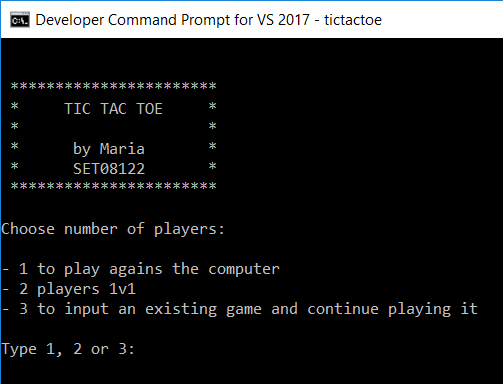
\includegraphics{images/1.png}
    \caption{Start of game}
    \label{fig:players}
\end{figure}

\begin{figure}
    \centering
    \includegraphics{images/2.png}
    \caption{Asking for player's names}
    \label{fig:names}
\end{figure}

\begin{figure}
    \centering
    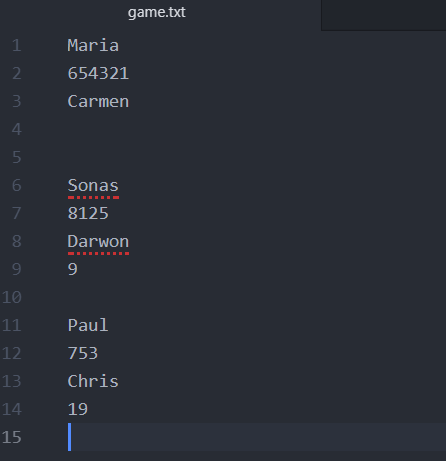
\includegraphics{images/game.png}
    \caption{Games history file, How all the games are saved}
    \label{fig:gameHistory}
\end{figure}

\begin{figure}
    \centering
    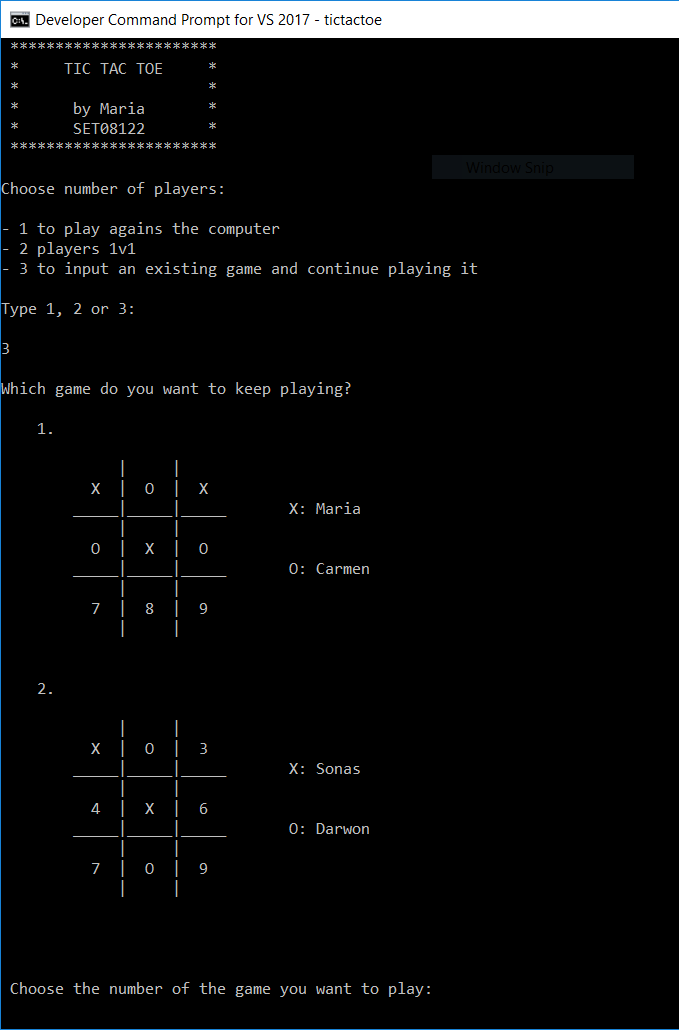
\includegraphics{images/choose.png}
    \caption{All games saved are displayed along with an ID number for the user to choose which game they want to continue playing}
    \label{fig:choose}
\end{figure}

\end{document}
